\documentclass[times, twoside, watermark]{zHenriquesLab-StyleBioRxiv}
\usepackage{blindtext}
\usepackage[htt]{hyphenat}
% Please give the surname of the lead author for the running footer
\leadauthor{BU} 

\begin{document}

\title{Interoperable Application for Issuing CIS Benchmarks }
\shorttitle{Interoperable CIS}


\author[1]{Mert Toslali}
\author[1]{Jonathan Chamberlain}
\author[1]{Felipe Dale Figeman}
\author[1]{Zhengyang Tang}

\affil[1]{BU EC528 - Cloud Computing}

\maketitle

%TC:break Abstract
%the command above serves to have a word count for the abstract
\begin{abstract}
The Open Container Initiative (OCI) has been established to create a open standard for container use regardless of the runtime being used to manage the container. However, the OCI only specifies downloading image then unpacking that image into an OCI Runtime filesystem bundle. It does not standardize lifecycle management of the containers, thus each container implements lifecycle functionality in a different manner. It also does not ensure that consistent standards for the security of containers are present.

In this project, we study the differences in popular runtimes Docker, containerd, and crio. Our focus is on developing an interoperable application focused on ensuring that Center for Internet Security (CIS) Benchmarks are satisfied across runtimes to ensure consistent application of security principles irrespective of container runtime differences. By implementing an application, which can be exposed as a service to validate standard security checks across runtimes, we intend to provide a Proof of Concept that such a common lifecycle management is possible.
\end {abstract}
%TC:break main
%the command above serves to have a word count for the abstract



\section*{Introduction}
\label{section:introduction}
Virtualization of resources has emerged in recent decades as a means to run multiple OSes on the same hardware. This particularly serves a useful function as this allows multiple applications to coexist on the same server, enabling efficencies in computing such as server consolidation.

Traditional VMs virtualize hardware resources, which results in the VMs taking up more resources. As such, OS-level virtualization, or Containers, have been developed. By sharing OS resources, containers are lightweight and can be spun up quickly while taking up fewer resources.
Sharing OS resources such as libraries significantly reduces the need to reproduce the operating system code, and means that a server can run multiple workloads with a single operating system installation.
Containers are thus exceptionally light.

Containers are implemented using Linux namespaces and cgroups. \textbf{Namespaces} let you virtualize system resources, like the file system or networking, for each container. \textbf{Cgroups} provide a way to limit the amount of resources like CPU and memory that each container can use. 


Docker, introduced in 2013, is a popular runtime to manage containers as it addresses end-to-end management. However, Docker was initially a monolith with features not inherently dependent on each other being bundled together. As a result, alternative runtimes such as CRI-O and contianerd exist which implement container management at varying levels. [1]

The Open Container Initiative (OCI, https://www.opencontainers.org) has been established to create a open standard for container use regardless of the runtime being used to manage the container. However, the OCI only specifies downloading image then unpacking that image into an OCI Runtime filesystem bundle.

It does not standardize lifecycle management of the containers, thus each container implements lifecycle functionality in a different manner. It also does not ensure that consistent standards for the security of containers are present.

In this project, we study the differences in popular runtimes Docker, containerd, and crio. We propose an interoperable application focused on ensuring that Center for Internet Security (CIS) Benchmarks are satisfied across runtimes to ensure consistent application of security principles irrespective of container runtime differences. By implementing an application, which can be exposed as a service to validate standard security checks across runtimes, we intend to provide a Proof of Concept that such a common lifecycle management is possible. Minimum viable product for this project was to implement 5 CIS benchmarks from chapter 5 over at least two different container runtimes. However, we go way beyond the MVP and implement 23 Benchmark checks for docker, 20 for crio, and 16 for containerd. Detailed implementation for the benchmarks can be found in later sections and appendix.  

\subsection{Vision and Goals}
Currently if someone wishes to launch an image in a container or perform any other lifecycle management functions on it, they must be sure that the scripts are configured correctly for the target container. For instance, launching images in Docker differs from doing so in crio or containerd. This locks individuals and businesses into whichever container runtime they started with unless they invest the time required to edit the configuration and their scripts which holds the commands for target container.

Our short term goal for this project is to enable the set of Container Runtime tests run in the CIS Docker 1.13.0 Benchmark across any container runtime. These tests are specified in Chapter 5 of the document; example checks include restricting Linux Kernel capabilities within containers, limiting memory usage, and avoiding directly exposing the host devices to the containers. Publishing a minimum viable framework for this purpose will enable users to run their security checks using a single application across the most popular containers.


\subsection*{Users/Personas of the Project}
The intended user is a software developer who is developing, testing or a security engineer who is managing applications and ensuring reliability across containers running on different runtimes.

Example Use Case: A software developer would like to launch an image in CRI-O instead of Docker, because he realizes that CRI-O is more adaptable with Kubernetes, and using this capability will provide this application a lot more scalability. Presently, he needs to deal with changing all the continous-integration scripts in order to be able to test and deploy his application on this new container runtime. With our interoperable framework in place, the developer is at least able to run security checks on the new container runtime with our application by specifying the new target container. In this way, the user's workflow is simplified and can apply a standard security checks across runtimes with minimal effort.

\subsection*{Scope}
The runtimes in scope for capability for this project will be Docker, and CRI-O. containerd is considered a runtime in scope as a stretch goal.

This project aims to ensure that the framework implements commands that satisfy the CIS Docker 1.13.0 Benchmark related to Container Runtimes across our in-scope runtimes. In doing so, users will be enabled to run their security checks with a single application rather than requiring separate suites for each runtime. The MVP is considered to be implementing at least 5 benchmarks in consultation with our mentor. Implementation of the full suite is a stretch goal.

These benchmarks are specified in pp 126-180 of the Benchmark documentation

\section*{Design}
As the intent is to examine containers and their associated images to validate they meet the security benchmarks, the Interopable Application and the Interoperable Image Application need exposure to the container and image configuration files, as well as sysfs and procfs. Thus, the applications are deployed on the cluster hosting the containers to be inspected, and exist between the user and the container.

The applications are implemented in Python version 3. At present, the applications are implemented as separate standalone scripts which are called with a specified runtime and container ID on the command line. This was done largely to provide proof of concept that performing the checks are possible, and to facilitate testing. Combining the applications into a single service is part of future work discussed in a later section.

In addition, there is a separate helper function, the Image Approval Manager that works with the Interoperable Image Application. This manager simply takes image ids and adds them to a list of approved images or blocked/unapproved images. This helps to facilitate one of the benchmark checks outlined in the section on container image benchmarks. 


\subsection*{Implications and Discussion}

Where possible, the Interoperable Application leverages the attributes that are exposed in \textit{sysfs} and \textit{procfs} per process in Linux. sysfs and proc are pseudo-filesystems which provide an interface to kernel data structures. The files under sysfs provide information about devices, kernel modules, filesystems, and other kernel components. For instance, sysfs provides a means to determine if memory usage has been limited, as well as if the CPU priority is set appropriately. proc is primarily used to determine if the AppArmor Profile is enabled for the associated process id. 

The use of these interfaces limits the possibility that future updates to the containers causes a change in the configuration file structure, which would then require an overhaul of the applications to ensure that the security checks can still be carried out for the impacted runtime. However, some attributes are only found in the configuration files. This is especially true for any attribute related to the image files. Thus, a major part of this project was dissecting how each runtime operates, and which configuration files are utilized. 



\subsection*{CIS Benchmarks}
CIS is a community driven organization of volunteer professionals, aimed at refining best practices and tools for information security \cite{CIS_Communities}. CIS publishes various Benchmark documents for best practices for secure configuration of systems, including Docker \cite{CIS_Benchmarks}. There are no specific Benchmark documents for cri-o and containerd, however the majority of the Docker benchmarks are concerned with attributes which are not Docker-specific. 

Thus, our design is focused on determining how the relevant setting or settings for each benchmark are enabled in each runtime, and validate that the benchmark is satisfied. As noted under the challenges section however, in many cases there is not an unambiguous pass condition, instead simply having a fail condition to check against. Where possible we highlighted instances that did not fail but do not necessarily follow a best practice highlighted elsewhere, or require manual follow up before being able to identify a pass/fail, as is the case with most of the image benchmarks.
\subsection*{CIS Chapter 5}
The ways in which a container is started governs a lot of security implications. It is possible
to provide potentially dangerous run-time parameters that might compromise the host and
other containers on the host. Verifying container run-time is thus very important. In this project we implement various
recommendations to assess the container run-time security that is provided through CIS Chapter 5.

We implement following benchmarks: 

 \subsubsection*{5.1 Do not disable AppArmor Profile (Scored)} 
AppArmor protects the Linux OS and applications from various threats by enforcing
security policy which is also known as AppArmor profile. You can create your own
AppArmor profile for containers or use the Docker's default AppArmor profile. This would
enforce security policies on the containers as defined in the profile.

\subsubsection*{5.2 Verify SELinux security options, if applicable (Scored)} SELinux provides a Mandatory Access Control (MAC) system that greatly augments the
default Discretionary Access Control (DAC) model. You can thus add an extra layer of safety
by enabling SELinux on your Linux host, if applicable.

\subsubsection*{5.3 Restrict Linux Kernel Capabilities within containers (Scored)} By default, Containers start with a restricted set of Linux Kernel Capabilities. It
means that any process may be granted the required capabilities instead of root access.
Using Linux Kernel Capabilities, the processes do not have to run as root for almost all the
specific areas where root privileges are usually needed. 
\begin{itemize}
    \item NET\_ADMIN
    \item SYS\_ADMIN
    \item SYS\_MODULE
\end{itemize}

\subsubsection*{5.6 Do not run ssh within containers (Scored)}Running SSH within the container increases the complexity of security management by
making it
difficult to manage access policies and security compliance for SSH server. Difficult to manage keys and passwords across various containers. Difficult to manage security upgrades for SSH server
It is possible to have shell access to a container without using SSH, the needlessly
increasing the complexity of security management should be avoided.


\subsubsection*{5.9 Do not share the host's network namespace (Scored)} This is potentially dangerous. It allows the container process to open low-numbered ports
like any other root process. It also allows the container to access network services like Dbus on the Docker host. Thus, a container process can potentially do unexpected things
such as shutting down the Docker host. You should not use this option.

\subsubsection*{5.10 Limit memory usage for container (Scored)}
By default, container can use all of the memory on the host. You can use memory limit
mechanism to prevent a denial of service arising from one container consuming all of the
host’s resources such that other containers on the same host cannot perform their intended
functions. Having no limit on memory can lead to issues where one container can easily
make the whole system unstable and as a result unusable.

\subsubsection*{5.11 Set container CPU priority appropriately (Scored)}
By default, CPU time is divided between containers equally. If it is desired, to control the
CPU time amongst the container instances, you can use CPU sharing feature. CPU sharing
allows to prioritize one container over the other and forbids the lower priority container to
claim CPU resources more often. This ensures that the high priority containers are served
better.

\subsubsection*{5.24 Confirm cgroup usage (Scored)} System administrators typically define cgroups under which containers are supposed to
run. 
At run-time, it is possible to attach to a different cgroup other than the one that was
expected to be used. This usage should be monitored and confirmed. By attaching to a
different cgroup than the one that is expected, excess permissions and resources might be
granted to the container and thus, can prove to be unsafe.

\subsubsection*{5.28 Use PIDs cgroup limit (Scored)} Attackers could launch a fork bomb with a single command inside the container. This fork
bomb can crash the entire system and requires a restart of the host to make the system
functional again. PIDs cgroup --pids-limit will prevent this kind of attacks by restricting
the number of forks that can happen inside a container at a given time.


\subsection*{CIS Chapter 4}
cis chapter 4 [Jonathan]





\section*{Interoperable Application}

The Interoperable Application is a Python executable, which accepts two parameters from user: the target container's runtime and the container-id. For instance, to evaluate the CIS Chapter 5 benchmarks over a Docker container with id = 0606, a user is expected to run the following command:
\texttt{./interoperable\_app --docker 0606}.

In this section we demonstrate that we are able to perform more than 10 benchmarks over all in-scope container run-times. For brevity, we highlight the benchmark check implementations that were more challenging. For the full list of benchmarks implemented per runtime, please refer to Figures \ref{fig:docker}, \ref{fig:crio}, and \ref{fig:containerd} in the Appendix.
\subsubsection*{Docker}
Our primary platform is Docker container run-time. Here, we evaluate the how we implement the CIS checks on Docker. 
First, we find target container's pid from \textit{/run/containerd/io.containerd.runtime.v1.linux/moby/}
\textit{<container-id>/init.pid}.
In order to issue \textbf{5.1 Do not disable AppArmor Profile} and \textbf{5.2 Verify SELinux security options} benchmarks over Docker, we use procfs and pid. Apparmor and SELinux are security attributes for a given process. So these values are stored under \textit{/proc/<pid>/attr/apparmor/current} and \textit{/proc/<pid>/attr/selinux/current} respectively. By exposing these values, we are able to issue \textbf{5.1} and \textbf{5.2}.

Per container instance, configuration file is created under \textit{/run/containerd/io.containerd.runtime.v1.linux/moby} \textit{/<container-id>/config.json} file. From this file, we get \textbf{cgroup} path of a given container. Exposing this value also corresponds to \textbf{5.24} benchmark.

Further, by using the cgroup path, we are able to access \textit{sysfs} of a given container. \textit{sysfs} is a pseudo file system provided by the Linux kernel that exports information about various kernel subsystems. From this file, we are able to perform \textbf{5.10, 5.11, 5.28}. \textbf{5.10 Memory Limit} of a container is found from: \textit{/sys/fs/cgroup/memory/<container-id>/memory.limit\_in\_bytes}.
\textbf{5.11 CPU Share} of a container is found from: \textit{/sys/fs/cgroup/cpu/<container-id>/cpu.shares}.
\textbf{5.28 PID Limits} of a container is found from: \textit{/sys/fs/cgroup/pids/<container-id>/pids.max}.
 
\subsubsection*{Containerd}


Other platform that we evaluate interoperable application is Containerd  run-time. The process for implementing given benchmarks are pretty similar to Docker that is
mentioned above. Since different runtimes comes with different configuration files and corresponding structures, we state the implementation details as following.
First, we find target container's pid from \textit{/run/containerd/io.containerd.runtime.v2.task/default/}
\textit{<container-id>/init.pid}.
In order to issue \textbf{5.1 Do not disable AppArmor Profile} and \textbf{5.2 Verify SELinux security options} benchmarks on Containerd, interoperable application
uses procfs and corresponding pid for a container. Apparmor and SELinux are security attributes for a given process. 
These values are stored under \textit{/proc/<pid>/attr/apparmor/current} and \textit{/proc/<pid>/attr/selinux/current} respectively. 
By exposing these values, we are able to issue \textbf{5.1} and \textbf{5.2}.

Per container instance, configuration file is on containerd created under \textit{/run/containerd/io.containerd.runtime.v2.task/default/} \textit{/<container-id>/config.json} file.
From this file, we get \textbf{cgroup} path of a given container. Exposing this value also corresponds to \textbf{5.24} benchmark.

Further, by using the cgroup path, we are able to access \textit{sysfs} and leverage attributes of a container. 
 From this file, we are able to perform \textbf{5.10, 5.11, 5.28}. 
 We specifically use followings:  \textbf{5.10 Memory Limit} of a container is found from: \textit{/sys/fs/cgroup/memory/<container-id>/memory.limit\_in\_bytes}.
\textbf{5.11 CPU Share} of a container is found from: \textit{/sys/fs/cgroup/cpu/<container-id>/cpu.shares}.
\textbf{5.28 PID Limits} of a container is found from: \textit{/sys/fs/cgroup/pids/<container-id>/pids.max}.
 
\subsubsection*{Cri-o}

Thus, we can see that the validation of our highlighted benchmarks is relatively similar across runtimes. This is largely because we are able to leverage the interfaces processed by sysfs and procfs to validate attributes associated to the container process. The principal challenge in the implementation was understanding where the relevant attributes necessary were stored, as well as understanding how sysfs and procfs work. As noted below, there exist other configuration files associated with containers which are used in validating the remaining benchmarks.

\subsection*{Other benchmarks}

In this section we briefly highlight how to validate the remaining benchmark checks impelmented for each runtime. The Benchmarks are refered to by their number as listed in \cite[Ch. 5]{center_for_internet_security}. The full list is contained in the Appendix, and as noted previously the associated scope for each benchmark is contained within the cited Benchmark document. 

For the remaining benchmarks, the Interoperable Application primarily leverages fields within the corresponding configuration files for the target container container. For example, to validate \textbf{5.4, 5.7, 5.8, 5.9, 5.12, 5.13, 5.14, 5.15, 5.16, 5.17, 5.18, 5.20 and 5.25} in Docker, we use Hostconfig.json file for a given container and inspect the relevant fields. For a particular container, this file is stored on the path: \textit{/var/lib/docker/containers/} \textit{<container-id>/hostconfig.json}. To implement checks for benchmarks \textbf{5.3, 5.5, 5.21, 5.24} in Docker, our application uses the config.json file located at \textit{/run/containerd/io.containerd.runtime.v1.linux/moby/} \textit{<container-id>/config.json}.
\\

For cri-o, the checks on benchmarks \textbf{5.3, 5.4, 5.5, 5.7, 5.8, 5.9, 5.12, 5.13, 5.15, 5.16, 5.17, 5.20, 5.21, 5.24} are implemented within the Interoperable Application by inspecting the container's config.json file. The relevant file is located on the path \textit{/var/lib/containers/storage/overlay-containers/}\textit{<container-id>/userdata/config.json}
\\

For containerd, the container's config.json file is again used to validate benchmarks. Specifically, the Interoperable Application is able to inspect relevant fields to validate \textbf{5.3, 5.4, 5.5, 5.17, 5.24, 5.25} using the config.json file per container.
This file is found on the path \textit{/run/containerd/io.containerd.runtime.v2.task/default//} \textit{<container-id>/config.json}.
The Interoperable Application inspects the container's state.json file in order to validate benchmarks \textbf{5.12, 5.15, 5.16, 5.20, 5.21}.
This file is located at \textit{/run/containerd/runc/default/}\textit{<container-id>/state.json}

\section*{Interoperable Image Application}

Currently, the validation on the image benchmarks is performed by a separate application. In addition to ensuring modularization of code, this was also done to prevent interference with the main Interoperable Application. Similarly to that application, the Interoperable Image Application is a python executable which takes the target container's runtime and the container id as input. Thus, if a user wishes to run the CIS Chapter 4 benchmark checks on the image running on container 0606, the user is expected to run the following:
\texttt{./interoperable\_image\_app --docker 0606}.

In this section, we demonstrate that we are able to evaluate at least some of the benchmarks discussed in the section on Container Images and Build File Benchmarks within Docker and cri-o, and how these are evaluated. 

\subsection*{Docker} Within Docker, each image has a configuration file corresponding to it located within the Docker image directory: \textit{/var/lib/docker/image/overlay2/imagedb/content/}
\textit{sha256/<image id>}. This file contains the attributes relevant to most of the benchmarks currently implemented.

To find the id of the image that a container is running, the application inspects the relevant configuration json for the image id: \textit{"/var/lib/docker/containers/}
\textit{<container id>/config.v2.json} The image id is a distinct attribute within this json file. 

Once opened, the application can validate benchmark \textbf{4.1, Create a user for the container} by determining if the User field is populated. If not, the user is root and the check fails. To validate benchmark \textbf{4.9, Use COPY instead of ADD in Dockerfile}, the Interoperable Image Application inspects the history attribute, which contains an entry for each instruction used to create the image. If any entry as ADD present, the benchmark is flagged as a failure; if a COPY instruction is present with no ADD instructions, the benchmark is marked as passing. If no ADD or COPY instructions are present, the bemchmark is flagged as not applicable rather than passing, as it is not clear this should be considered a pass based on the wording of the recommendation. This is a design decision which may be changed based on future feedback on best practices.

To validate benchmark \textbf{4.6, Add HEALTHCHECK instruction to the container image}, the application checks the image configuration file to determine if the healthcheck attribute is present. If not, the check is flagged as a failure. If an instruction is present, it is flagged as a pass unless the curl or iwr instruction is detected. In that case, the benchmark is flagged as requiring further follow up. This is because there may be additional dependencies required for these instructions to function properly in the associated container.

The remaining benchmarks do not require the image configuration file. To validate benchmark \textbf{4.5, Enable Content trust for Docker}, the application checks if the environment variable ENABLE\_DOCKER\_TRUST is set to 1. If so, the benchmark passes. If not set or set to any other value, the benchmark fails.

To validate benchmark \textbf{4.2, Use trusted base images for containers}, the application checks the image id against a pair of lists: an approved list and a block list. If the id is found in the approved list, the benchmark passes. If the id is found in the block list, the benchmark is rejected. If the image id is found in neither list, it is flagged for further follow up, as in this case it is considered to be an unknown image. This requires follow up by a System Administrator or a security officer to ensure the provencence of the image. Based on this follow up the image can be added to the approved list or block list as appropriate using the Image Approval Manager.

\subsection*{cri-o} Within cri-o, we adopt a reduced set of these checks, in part due to differences in the configuration files. Of the attributes discussed in the previous section, only the history is contained in the manifest file related to the target image. However, the user being used by the container is contained in the \textit{container's} configuration json file.

Thus, to validate benchmark \textbf{4.1} in cri-o, the Interoperable Image App simply inspects the user attribute in the container config.json located at \textit{/var/lib/containers/storage/overlay-containers/}
\textit{<container id>/userdata/config.json}. If the associated uid is 0, the check fails as 0 is the root user id. Otherwise, the check passes as a non root user is present.

The same configuration file contains an id within the image attribute. However, this is not the id associated with the image manifest but rather a digest hash. In order to solve this additional layer of indirection, the Interoperable Image App first opens the images.json file within the overlay-images directory: \textit{/var/lib/containers/storage/}
\textit{overlay-images/images.json} This file contains information about all images, including the association between the image id, and the image digest stored in the image configuration file.

Once a matching id is found, the application is able to open the corresponding manifest file: \textit{/var/lib/containers/storage/}
\textit{overlay-images/<image id>/manifest}, and inspect the history attribute in order to validate benchmark \textbf{4.9}. In addition, with the image id known benchmark \textbf{4.2} is verifiable in the same manner as in Docker.

Currently, validation of the benchmarks \textbf{4.5, Enable Content trust for Docker} and \textbf{4.6, Add HEALTHCHECK instruction to the container image} are not currently implemented for cri-o by the Interoperable Image Application. In the case of the former, this is because signature verification for image content trust in cri-o is handled by a policy.json file and does not involve setting an enviornment variable as in Docker. The policy.json file allows for a refinement of policies based on the source in question. While this allows acceptance/rejection based on specific criteria, a global default is required, which is frequently set to insecureAcceptAnything which does not reject anything. \cite{containerd_policy_json}. To properly implement this particular check requires additional feedback as to best practices.

For the latter, there exists a code module within libpod to perform healthchecks on containers \cite{healthcheck_crio}. It is not clear based on this how to validate the Healthcheck instructions, as there is no guidance as to where the module is looking for the check as defined by the container. Thus, further followup is required to determine how to leverage this check within cri-o.

\subsubsection*{containerd} Currently, the Interoperable Image Application is not implemented within containerd. While we determined the location of the configuration file contianing relevant attributes, \textit{/var/lib/containerd/io.containerd.content.v1.content/}
\textit{blobs/sha256}, there is no attribute in the known configuration files for the container that links the container to the image id in such a way that we can know which image to run the checks on. This was filed as work for future follow up in order to avoid stalling progress on the other runtimes.

\section*{Challenges and Take Aways}

The primary challenge up front was figuring out how the runtimes operate. In particular, frakti was initially part of our in-scope runtimes. While relatively new, it is also in popular use per our mentor at IBM. However, documentation on how to install and run frakti proved to be outdated or otherwise incomplete. It is also not altogether clear whether frakti remains active as sources discussion other containers mention it primarily in passing. As a result, it was decided to remove frakti from scope due to insufficient information and it possibly being deprecated. This did result in wasted person-hours during the initial phase of the project in determining how the targeted runtimes operate.

With respect to implementing the benchmark checks, while verifying that a particular benchmark is not satisfied is fairly straightforward, there exists a parallel issue of the benchmarks not necessarily defining a best practice for what the setting should be set to. There is some logic to this - while what not to do is relatively straightforward to assess, such as flagging a container which does \emph{not} have a memory limit set, what limit should be placed on the container depends on organizational policy and what application the container is running. Thus, while finding the setting within the file is straightforward, whether there should be a means to set a threshold corresponding to institutional policy requires further discussion regarding how best practices should work.

This is especially the case for the benchmarks relating to the images, as many of the checks require manual follow up rather than being able to flag that a setting is missed. For instance, benchmark \textbf{4.3, Do not install unnecessary packages in the container} depends in part on what application the image is intended to be running. Other of the image checks require more complex logic in order to validate whether they pass or not, such as verifying whether only verified packages are installed (\textbf{4.11}), or using update instructions alone in the Dockerfile (\textbf{4.7}). 

The biggest take aways as a result are that there is not necessarily a standard value that the various attributes should be set to. In many cases, this can result in a default value which is dangerous for use on live containers. In relying on organizations to set the attributes themselves, this opens the containers and associated images to various attacks including fork bombs which can bring down the host, and infection of cgroups which can lead to exfiltration of container data by taking over kubernetes nodes \cite{aqua_blog}. However, there do exist built in isolation measures which can aid in preventing a single compromised container from creating issues for the other containers on the same host. Thus, the ability to verify whether those isolation measures are active (e.g. AppArmor, SELinux) is critical to container security.

In addition, another take away from the group as a whole is that once we were able to begin development, we became so caught up in checking off each benchmark as complete, that we failed to stop and reconsider the intended use case. In particular, whether the user we originally envisioned, a developer working with multiple runtimes, was the relevant one as the project evolved to primarily encompass running the security checks within each in-scope runtime. Upon feedback from the instructors, we took this back to our mentor who clarified that this is a tool to be leveraged by the CISO. However, at this point there was little time remaining to perform any additional changes to existing code to facilitate the next steps which emerged from that discussion, which leads us to our concluding section.

\section*{Future Work}

Currently the application requires manual invocation of a particular container on the command line. As our intended user is an organization CISO or their designated security personnel, this is not practical given that within a large organization, containers are spun up and stood down at large volumes, and thus it is not practical to inspect containers one by one. Thus, the current state of our application can be considered as being in more of a proof of concept stage, in that we can run checks for the majority of the specified benchmarks on a given container.

Given the number of containers to inspect, how to ensure scalability to efficiently report on each container is the next step to be considered. We imagine standing up a daemon running on a Kubernetes cluster. As containers are spun up, the daemon would be triggered and automatically run all of the benchmark checks. Reports would be made available to the designated security staff, with alerts if failures are detected or follow ups required (depending on the benchmark and result). One advantage is that all containers on the same cluster would utilize the same runtime, avoiding the need to specify the target runtime on each invocation. Ideally, it would be possible for this daemon service to automatically detect which runtimes are being used, however at present it is not clear how to do so, and thus for the moment it would be necessary to specify this on a configuration level.

In addition, there are still some benchmarks checks which have yet to be implemented. Given the nature of some of the benchmarks, both currently implemented and not, ideally there would be discussions with stakeholders as how to define a best practice in terms of what settings should be specifically set to (as opposed to specifying that they must be set at all). This would require a means to maintain a configuration to define the best practice as defined by a particular organization, one that is more robust than the currently implemented tool to manage approved/blocked images.

\section*{Bibliography}

\bibliography{interoperable}

\section*{Appendix}

\subsection*{Container Runtime Benchmark Recommendations} Below is the full list of benchmarks as listed in Chapter 5 of \cite{center_for_internet_security}, and as referenced by benchmark id in the Ineroparable Application section.

\begin{itemize}
    \item 5.1 Do not disable AppArmor Profile 
    \item 5.2 Verify SELinux security options, if applicable 
    \item 5.3 Restrict Linux Kernel Capabilities within containers 
    \item 5.4 Do not use privileged containers 
    \item 5.5 Do not mount sensitive host system directories on containers
    \item 5.6 Do not run ssh within containers 
    \item 5.7 Do not map privileged ports within containers 
    \item 5.8 Open only needed ports on container 
    \item 5.9 Do not share the host's network namespace 
    \item 5.10 Limit memory usage for container 
    \item 5.11 Set container CPU priority appropriately 
    \item 5.12 Mount container's root filesystem as read only 
    \item 5.13 Bind incoming container traffic to a specific host interface 
    \item 5.14 Set the 'on-failure' container restart policy to 5 
    \item 5.15 Do not share the host's process namespace 
    \item 5.16 Do not share the host's IPC namespace 
    \item 5.17 Do not directly expose host devices to containers
    \item 5.18 Override default ulimit at runtime only if needed 
    \item 5.19 Do not set mount propagation mode to shared
    \item 5.20 Do not share the host's UTS namespace 
    \item 5.21 Do not disable default seccomp profile 
    \item 5.22 Do not docker exec commands with privileged option 
    \item 5.23 Do not docker exec commands with user option 
    \item 5.24 Confirm cgroup usage 
    \item 5.25 Restrict container from acquiring additional privileges 
    \item 5.26 Check container health at runtime 
    \item 5.27 Ensure docker commands always get the latest version of the image 
    \item 5.28 Use PIDs cgroup limit 
    \item 5.29 Do not use Docker's default bridge docker0 
    \item 5.30 Do not share the host's user namespaces 
    \item 5.31 Do not mount the Docker socket inside any containers 
\end{itemize}




\begin{figure*}
    \caption{Benchmarks implemented in Docker.}
    \centering
      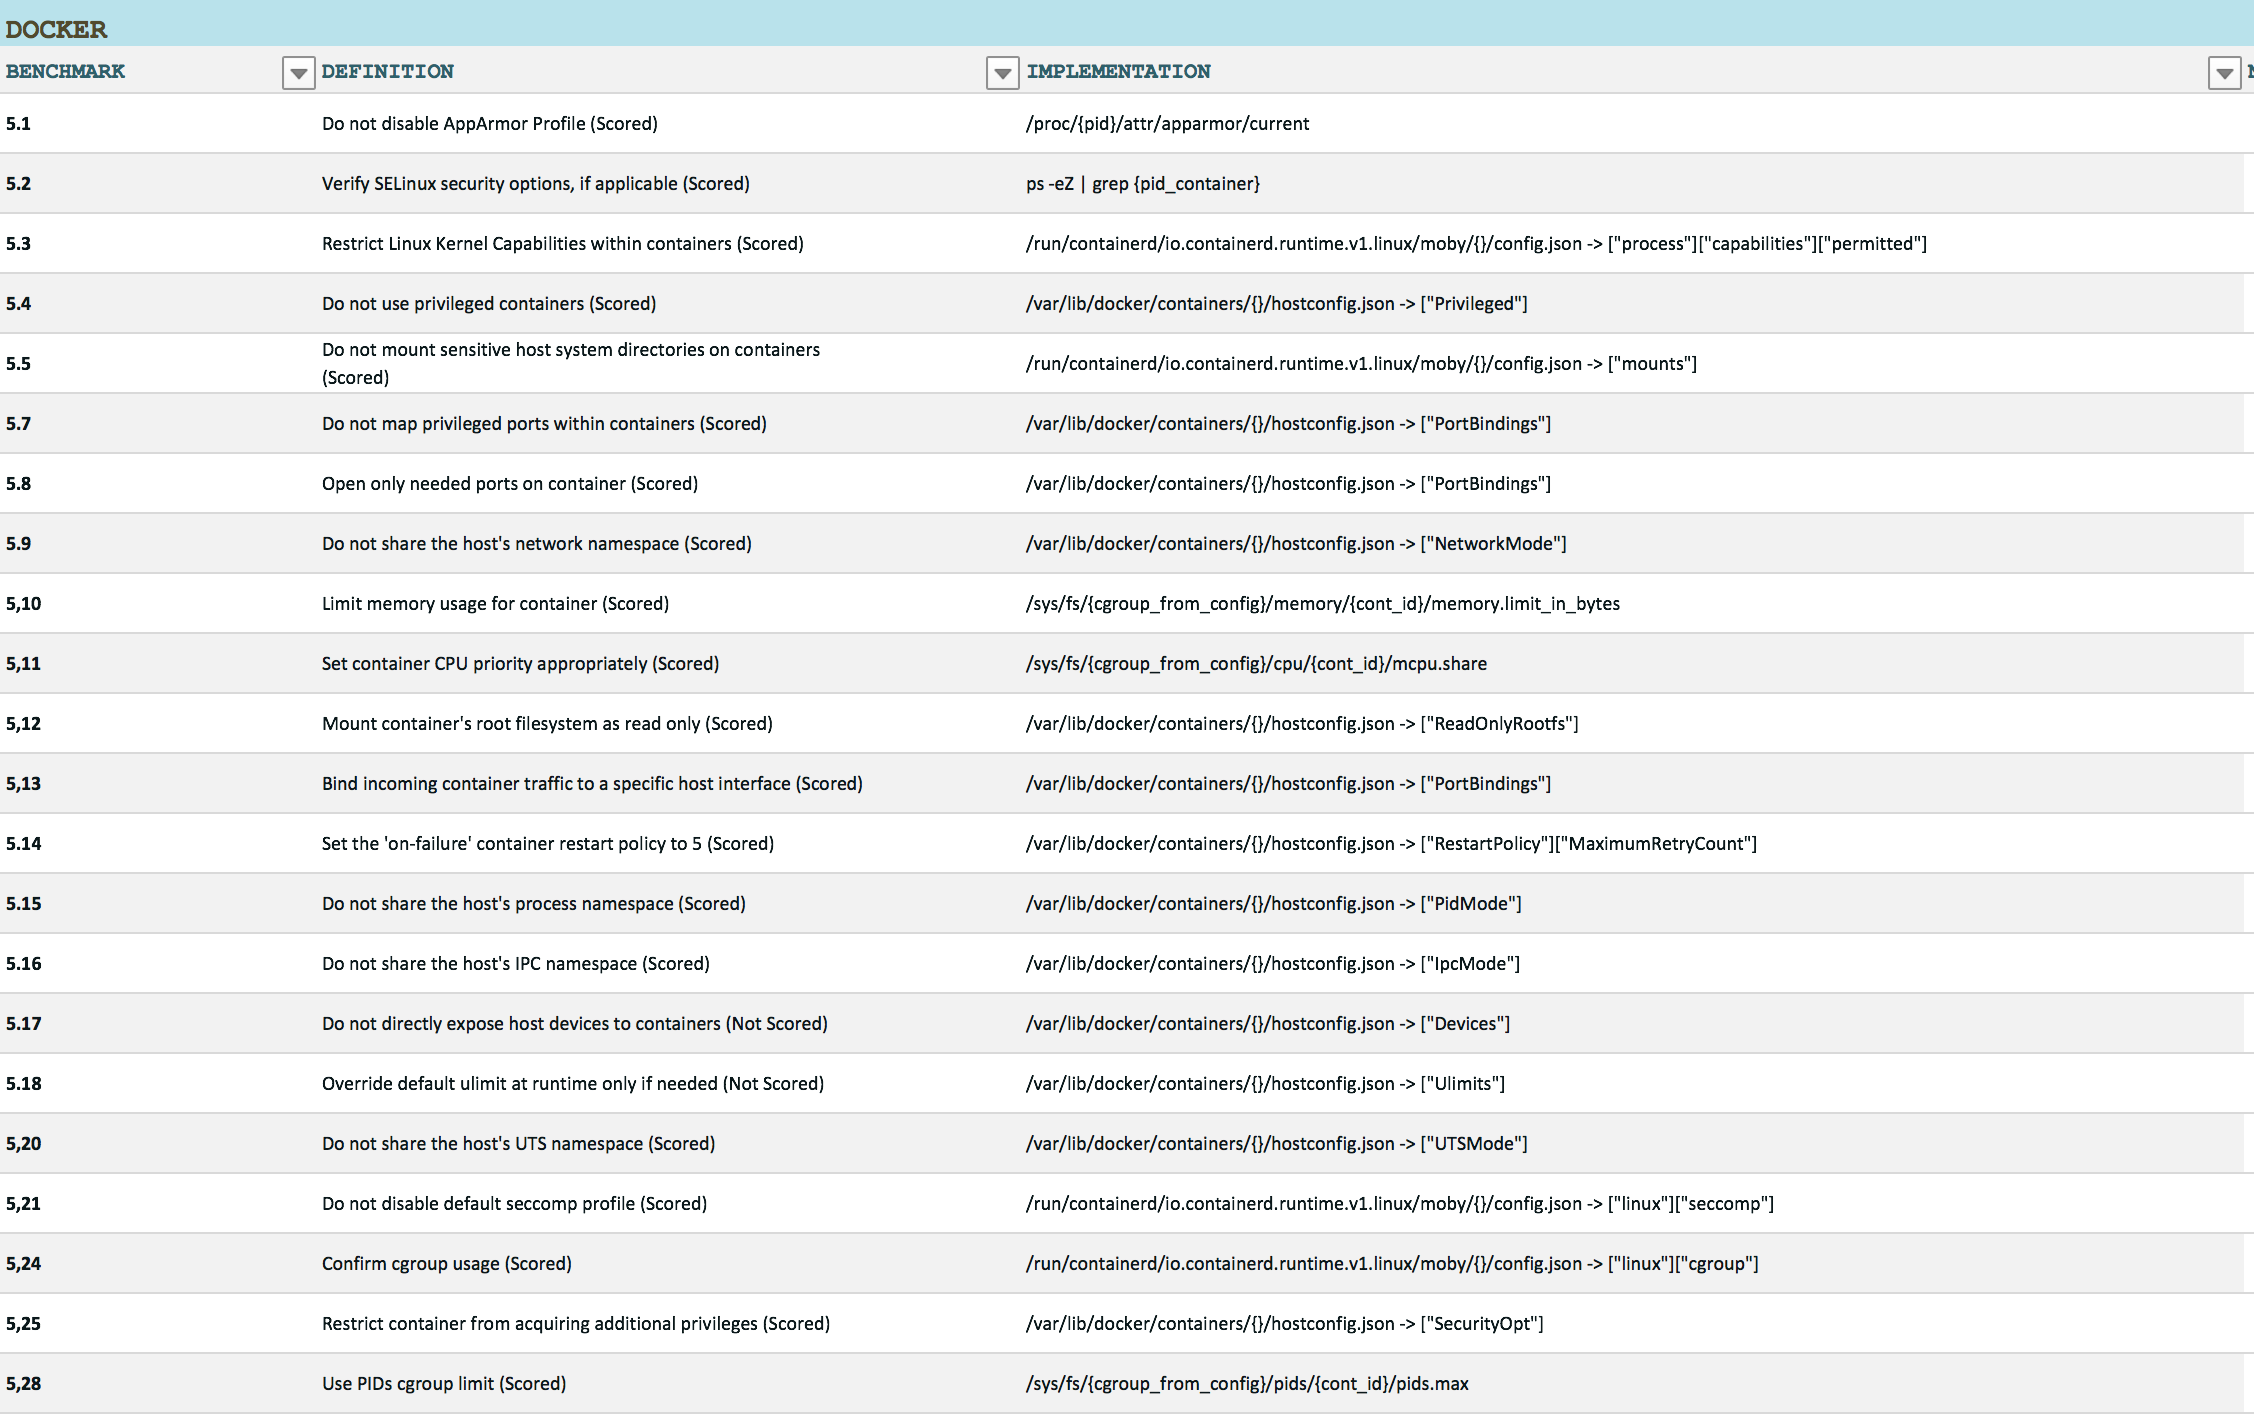
\includegraphics[width=\textwidth,height=10cm]{figures/docker}
      \label{fig:docker}
  \end{figure*}


  \begin{figure*}
    \caption{Benchmarks implemented in cri-o.}
    \centering
      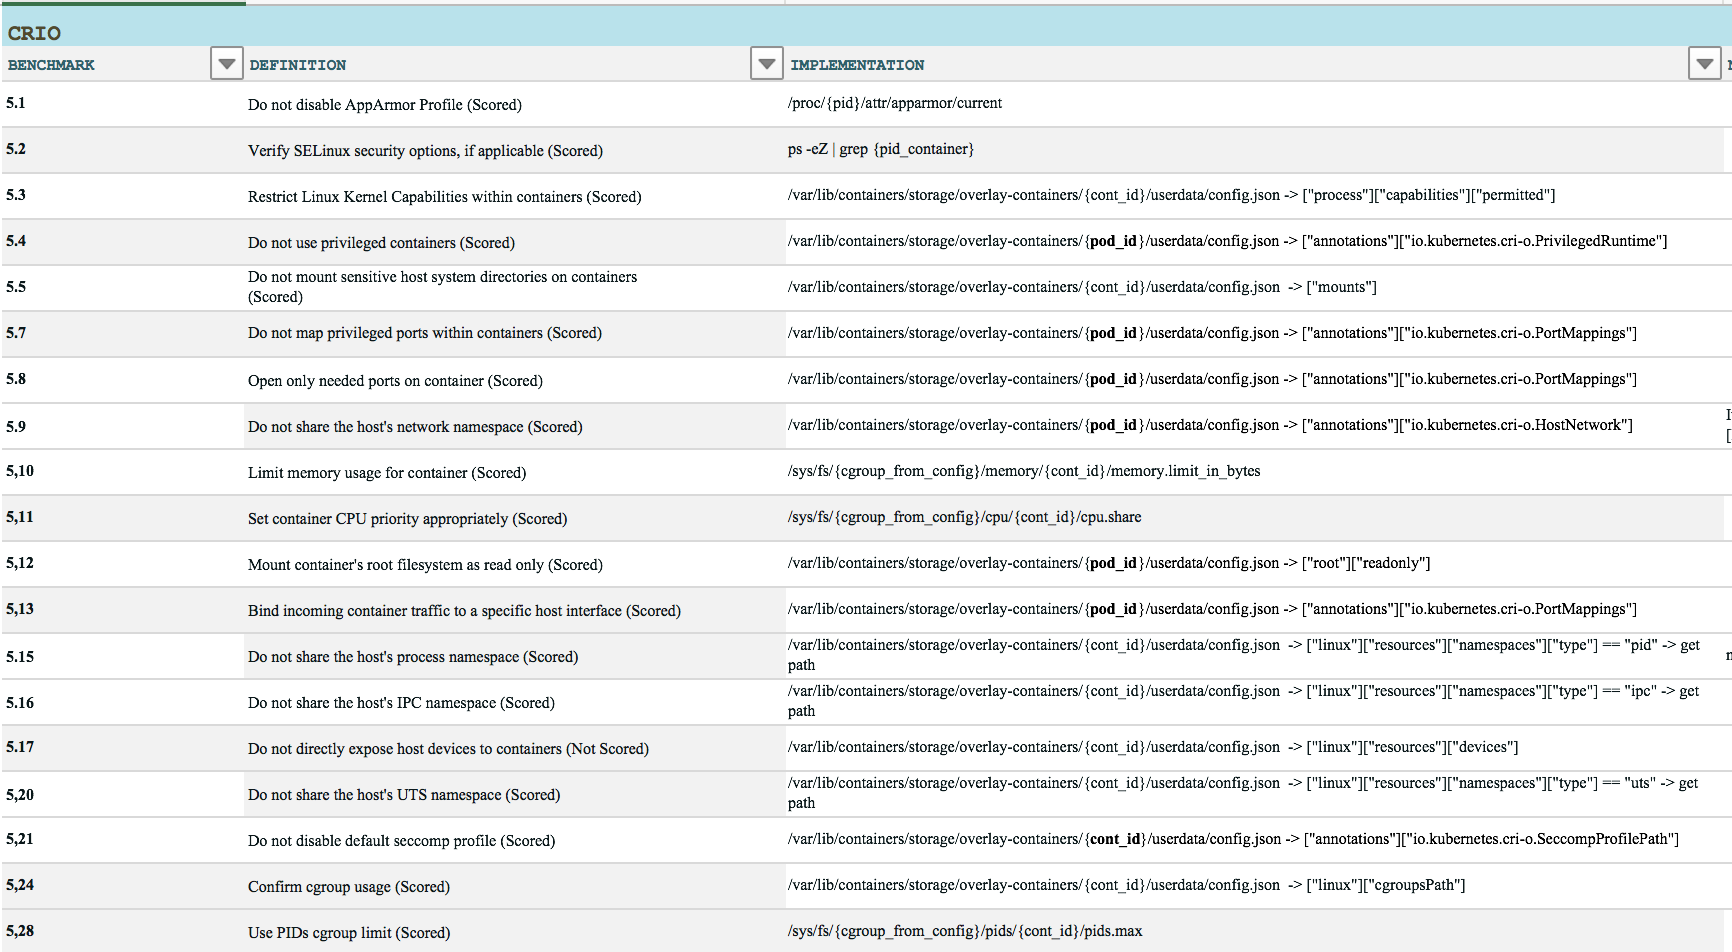
\includegraphics[width=\textwidth,height=10cm]{figures/crio}
      \label{fig:crio}
  \end{figure*}


  \begin{figure*}
    \caption{Benchmarks implemented in containerd.}
    \centering
      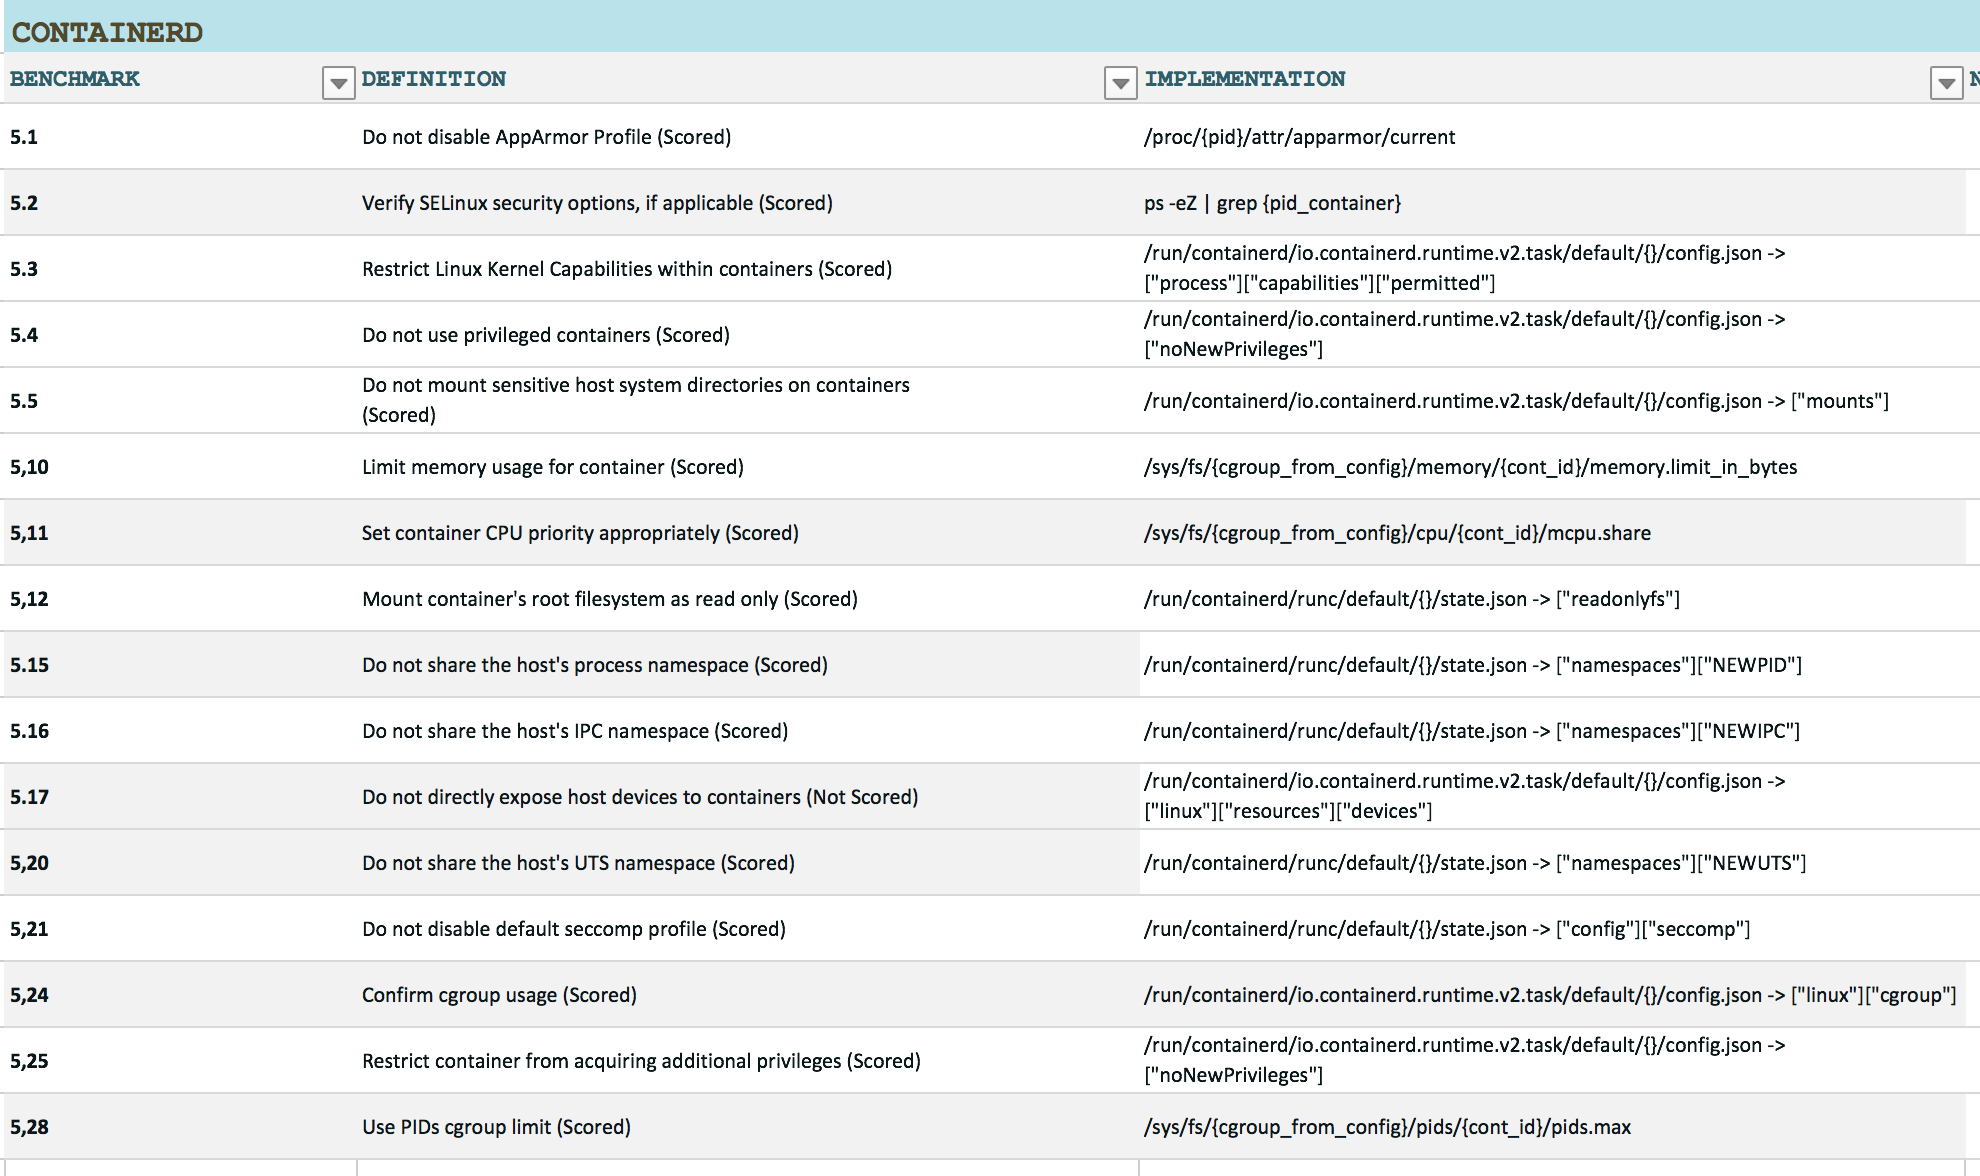
\includegraphics[width=\textwidth,height=10cm]{figures/containerd}
      \label{fig:containerd}
  \end{figure*}
  
  \begin{figure*}
    \caption{Partial Example of output from the Interoperable Application on a Docker container image}
    \centering
      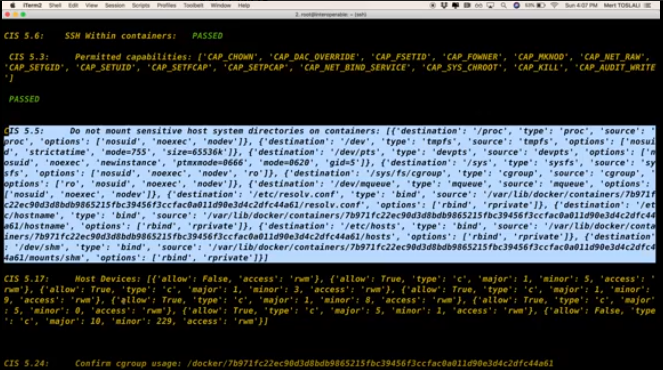
\includegraphics[]{figures/docker_interop_example.png}
      \label{fig:containerd}
  \end{figure*}

    \begin{figure*}
    \caption{Example of output from the Interoperable Image Application on a Docker container image}
    \centering
      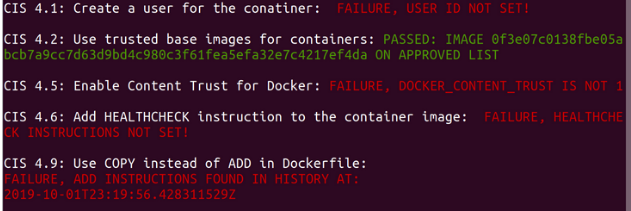
\includegraphics[]{figures/docker_interop_image_example.png}
      \label{fig:containerd}
  \end{figure*}

\end{document}
